\chapter{腹侧前额叶皮层:基于视听内容生成目标}
这本书提出了关于灵长类动物前额叶皮层基本功能的方案。
腹侧 PF 皮层根据视觉和听觉线索生成目标,我们称之为标志,它的连接解释了为什么只有它才能做到这一点。腹侧 PF 皮层与颞下皮层的视觉区和颞上皮层的听觉区以及其他PF区有联系。它与颞叶皮层的连接提供了视觉和听觉信号,从而建立了当前的行为环境。眼眶 PF 皮层提供了选择和结果之间的联系,有时可以在单个事件的基础上学习(第4章)。在许多任务中,腹侧 PF 皮层根据具体物体和地点生成目标。然而,在涉及抽象规则和策略的任务中,腹侧PF皮层可以生成一组或几类目标以供选择或避免。鉴于腹侧PF皮层在类人猿灵长类动物中进化第2章),我们认为它在使用视觉标志和声音信息方面具有优势,可以指导近距离和远距离的觅食选择。
\section{介绍}
\par
正如第 2 章所指出的,人们经常将灵长类动物描述为“视觉动物”。原因是中央凹在早期的单鼻科动物中进化,而三色视觉在类人猿中进化。 这些进步使这些动物及其后代能够辨别位置、颜色、形状、视觉纹理、光泽度和半透明度的微小差异。本章回顾了类人猿使用这些视觉特征来提供觅食机会线索的证据,我们称之为标志。正如第2章所解释的那样,我们所说的符号是指用作提示但不一定对应于整个对象的非空间景象和声音。
\par
进化已经设计出许多方法来获得觅食优势。一些哺乳动物通过精心制作身体部位来开发资源,从而利用了它们的生态位。大象的长鼻子使它们能够以其他哺乳动物无法做到的方式觅食。长颈鹿的长脖子同样提供了独特的觅食机会。我们认为,类人猿反而精心设计了某些大脑结构,包括腹侧PF皮层。
\begin{figure}
	\centering
	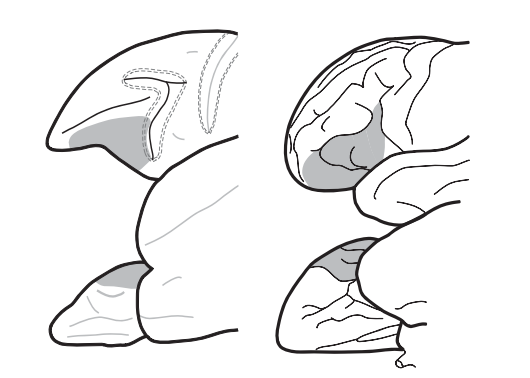
\includegraphics[width=0.7\linewidth]{image_pfc/Fig_7_1}
	\caption{猕猴(左)和人类(右)的腹侧PF皮层。格式如图1.2所示。}
	\label{fig:fig}
\end{figure}
\par
前一章解释了背侧PF皮层生成适合当前上下文的目标,如最近事件指定的,尤其是视觉事件。它解释了视觉线索的顺序、位置和时间的重要性,以及其他特征,强调与后顶叶皮层的联系。腹侧PF皮层与下颞叶皮层和上颞叶皮层相连。因此,可见或可听的标志也指定了当前的上下文,类人猿可以单独使用或结合由顺序、位置和时间确定的上下文使用。
\section{区域}
\par
在猕猴中,腹侧PF皮层包括主沟腹侧半球的外侧凸起(图 7.1)。在人类中,同源区域位于额下回。在两者中,腹侧PF皮层围绕半球的外侧末端延伸至外侧眶沟。术语12/47由Petrides和Pandya设计,反映了他们认为人类的47区与猴子的12区同源的观点 (Petrides\&Pandya 2002b)。
\par
就细胞结构区域而言,腹侧PF皮层包括猕猴的45区和12/47区(见图 1.2)。在人类中,腹侧PF皮层包括区域45和47。
\section{连接}
\begin{figure}
	\centering
	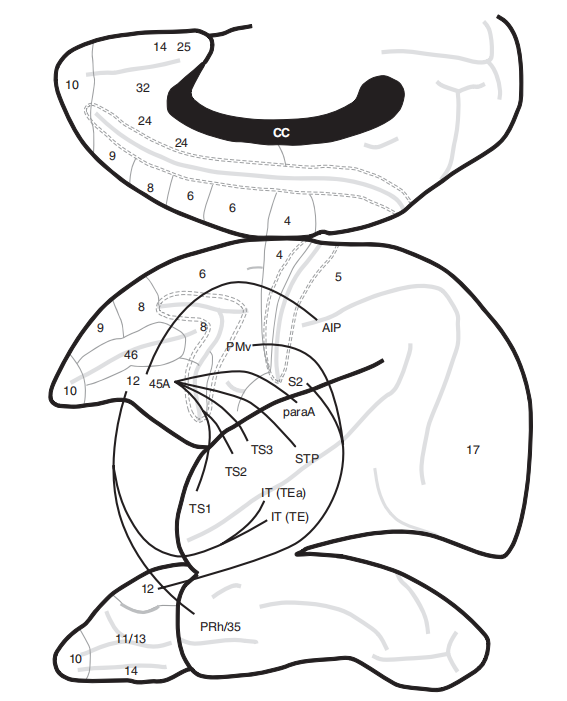
\includegraphics[width=0.7\linewidth]{image_pfc/Fig_7_2}
	\caption{腹侧PF皮层的选定连接。图1.4和1.5给出了脑沟和区域的名称。线连接一些与腹侧PF皮层具有直接轴突连接的区域,除非另有说明,否则假定它们是相互的。}
	\label{fig:fig}
\end{figure}
图7.2显示了腹侧PF皮质的皮质皮质连接。有几个特点很突出:
\par
1.如前所述,腹侧PF皮层与颞叶紧密相连。腹侧PF皮层与下颞叶皮层相互联系。格式如图1.2所示。连接197(Ungerleider 等人 1989;Webster 等 1994)和颞上皮层Seltzer等人1996年;Petrides \&Pandya 2002b)。它也与鼻周皮质有联系 (Suzuki \& Amaral 1994 ; Saleem et.al 2008),尽管没有那么多。 
\par
这些联系有两个含义。首先,腹侧PF接收有关指定行为环境的信号或标志的信息。下颞叶皮层在辨别颜色、形状和视觉纹理方面起着至关重要的作用 (Huxlin等人2000)。颞上皮层参与声音识别 (Tian 等人 2001) 和声音序列 (Micheyl et al. 2005),包括其他动物的叫声 (Rauschecker et al. 1995)。 
\par
其次,到达腹侧PF皮层的信息来自高级和中级视觉区域,而不是来自低级视觉区域。 通过高阶视觉,我们指的是一个物体特征的广泛结合,这是鼻周皮质所代表的 (Murray et al. 2007)。相比之下,下颞区,如TE区,构建了介于整个对象的表示及其基本特征之间的中级连词 (Murray et al. 2007)。 最尾部的视觉区域构建低阶连词,一些代表基本特征,但这些区域不投射到腹侧PF皮层(Webster 等人,1994 年)。在这方面,腹侧PF皮层的连接与尾侧PF皮层的连接不同(第 5 章)。
\par
2.腹侧PF皮层还与第二体感区 (S2) 附近的一组复杂区域相互连接 (Petrides \& Pandya 2002b)。 因此,腹侧PF皮层接收来自视觉、听觉和躯体感觉皮层的多模式输入。S2内部和周围的皮层有助于物体的触觉辨别 (Mishkin 1979),而鼻周皮层对于通过视觉或触觉识别物体至关重要 (Goulet \& Murray 2001;Murray 等人 2007)。
\par
3.腹侧PF皮层接收来自下顶叶区PG的输入 (Petrides \& Pandya 2002b)。此连接可能会提供有关对象位置的信息。腹侧PF皮层还接收来自后顶叶区域AIP的输入,这似乎在猴子拾起物体时使用视觉来校准抓握方面发挥作用(Fogassi 等人,2001 年)。
\par
4.腹侧 PF 皮层(区域 12/47)与腹侧前运动皮层的延髓部分有很强的联系。 最近的一份报告称这部分运动前皮层区域为 F5a(Gerbella 等人,2011年),第2章提到该区域似乎控制手和嘴的运动。 
\par
5.腹侧 PF 皮层也与杏仁核有关。 一些神经解剖学迷雾将这些描述为广泛的(Amaral \& Price 1984 ;Stefanacci \& Amaral 2002 年),但其他人认为它们稀疏(Carmichael \& Price 1995a;Price \& Drevets 2010)。无论如何,与杏仁核的连接可能会提供更新的估值,如第3章和第4章所解释的那样,直接连接到腹侧 PF皮层或通过眼眶PF皮层间接连接。包括下颞叶皮层(Horel 等人 1975 年)或杏仁核(Horel 等人 1975 年;Aggleton \& Passingham 1981 年)在内的损伤会影响物体看起来有吸引力还是令人厌恶,并且两者都与腹侧 PF 皮层有关。
\section{视觉和听觉条件任务}

\section{视觉空间和视觉运动协会}

\section{样本匹配任务}

\section{分类}

\section{抽象规则}

\section{改变规则}

\section{抽象策略}

\subsection{结论}


